\section{Background}
%Before discussing the new and significant elements that make Mini-MAC a valid security protocol for the CAN bus, there is some necessary background information that must be understood. \textcolor{red}{Note to ed: -- Not sure what goes well here.}

This section briefly reviews essential background on vehicular security and Message Authentication Codes. The experienced reader may wish to skip to section 3.

\subsection{ECUs}
The electronic control units found in an automotive computer network are low power, single purpose devices. ECUs on the CAN bus control many things in a modern automobile, from headlights and window controls to the brakes and engine. They are not typically designed with security in mind and frequently comprise a basic CAN bus transceiver, basic message processor, and an actuator. The message processor identifies whether or not a message being broadcast is interesting to the ECU and arbitrates bus rights with the other ECUs. %For testing for this project, a Texas Instruments MSP430F5529 microcontroller serves as a hardware platform for test code. The MSP430F5529 is a low-power, low-speed, low-cost MCU that is representative of the message processor present in an ECU.


\subsection{The CAN Bus}
The CAN bus is a simple, low-speed bus designed to network simple nodes. In an automotive environment, it typically runs at 500 kbps. A message contains an 11-bit identifier field and an 8-byte data payload as well as some control bits. Figure 1 illustrates a CAN packet. The 8-byte payload is the most important number, as any MAC must fit into this frame or use a more complex multi-frame data transmission protocol that may or may not be supported on all ECUs. Ideally, and in the case of Mini-MAC, the MAC can fit into the payload with the data, thus not increasing bus utilization. Data show that a large amount of messages (~61\%) use no more than 4-byte of data in the payload.

	\begin{figure}
		\centering
		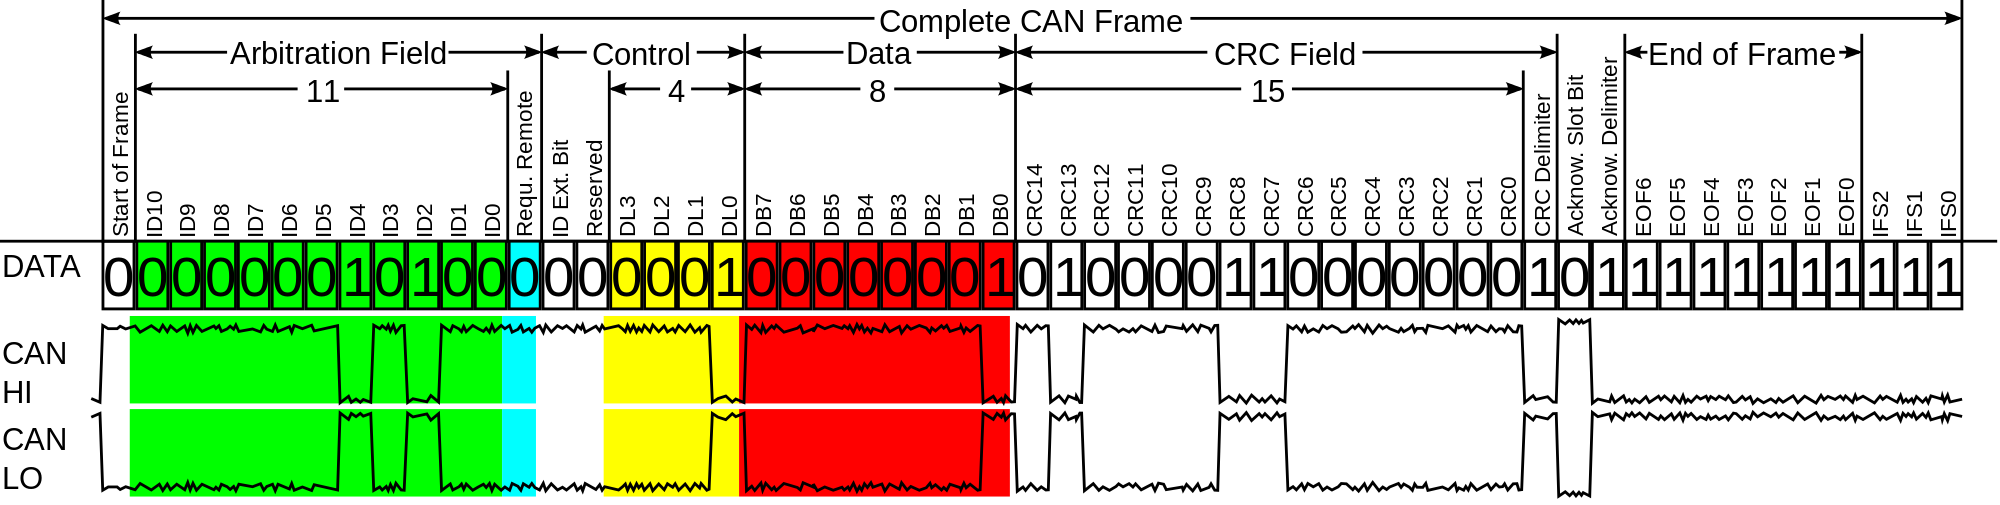
\includegraphics[width=\columnwidth]{figures/can_frame.png}
		\caption{CAN Frame}
	\end{figure}

\subsection{Bus Access}
%Manufacturers have noted that they see the threat to a vehicle presented by vulnerabilities stemming from the insecure CAN bus as unlikely to manifest due to the difficulty of getting access to the bus. 

Despite many demonstrated examples, automotive manufacturers are hesitant to acknowledge the vulnerabilities inherent to the CAN bus because of the difficulty in gaining access to it. It can be difficult -- the most typical way to gain access is through a physical connection through the On-Board Diagnostic port (OBD-II), which is located underneath the steering wheel. A driver might notice some kind of hardware module sticking out from underneath the wheel. It has been shown that it is possible, however, to gain remote access to these vehicles (or to corrupt / rewrite firmware on an ECU) through wireless channels such as the cellular modem or bluetooth radio. Researchers have even demonstrated gaining bus access by packing code into a WMA audio file played on the car stereo \cite{Checkoway-2011}.

\textcolor{red}{I saw your note on this subsection, but I think it's important to keep a mention of the work done in remote access here. I don't want to discuss that work on its own as it isn't related except that it helps show there are multiple paths to getting access to the CAN bus. What do you think?}

\subsection{Message Authentication Codes}
%The best solution, in that it is implementable and does not change the network infrastructure, to preventing replay and masquerade attacks on the CAN bus to this point is the work presented in Lin-MAC. The underlying MAC protocol was not described, however, and as the ECUs on this node are time-, memory-, and processing power-constrained, some testing must be done to determine which construction is the most suitable for the environment. 

Message Authentication Codes (MACs) are bit strings used to verify the identity of the sender in order to check the legitimacy of a message. These codes are usually relatively small compared to the length of the message. 

%HMAC is by far the most famous and most popular MAC construction, so three variants of HMAC (that is, HMAC with three underlying keyed-hash functions) were selected for consideration for this project. HMAC is widely used for two key reasons. 1) The security of HMAC is mathematically related to the security of the underlying hash function, which makes it relatively easy to trust and 2) it is extremely easy to plug in various hash functions, making it easy to update to a new implementation if issues are found in the currently used hash\cite{HMAC}\cite{FIPS-198-1}. They are implemented in C on the MSP430.

The Keyed-Hash Message Authentication Code (HMAC) is by the far the most famous and most popular MAC construction protocol. It is so widely used for 2 key reasons. 1) The security of HMAC is mathematically related to the security of the underlying hash function, which makes it relatively easy to trust and 2) it is extremely easy to plug in various hash functions, making it easy to update to a new implementation if issues are found in the currently used hash\cite{HMAC}\cite{FIPS-198-1}.

The equation for calculating the HMAC is as follows: 

$$ \text{HMAC} = H((K_0\oplus \text{opad})\vee H((K_0\oplus \text{ipad})\vee \text{message}) $$

Where $K_0$ represents the key, which is sized depending on the underlying hash, and opad and ipad are the outer and inner hash padding strings respectively. These strings are constant strings represented by 0x5C and 0x36 repeated until the hash input string is of the appropriate size. The term $H$ represents the hash function used to generate the HMAC. The symbols $\oplus$ and $\vee$ represent the XOR operation and concatenation respectively. \cite{FIPS-198-1}

\subsection{Car-to-X}
The Car-to-X network is the collection of vehicles, buildings, signs and road infrastructure that are connected to each other to enable more efficient traffic control and congestion relief. These networks are currently in fledgling states at best but will become more prevalent over time.